\documentclass[a4paper,11pt]{article} %ADD diffusion OR archiv for final versions
\usepackage[francais]{babel}
\usepackage[utf8]{inputenc}
\usepackage[T1]{fontenc}
\usepackage[margin=20mm,includeheadfoot,bindingoffset=5mm]{geometry}
\usepackage{mathtools}
\usepackage{amsfonts}
\usepackage{amssymb}
\usepackage{textcomp}
\usepackage{graphicx}
\usepackage[many]{tcolorbox}
\usepackage{epstopdf}
\usepackage{xcolor}
\usepackage{bm}
\usepackage{cases}
\usepackage{xspace}
\usepackage{lmodern}

%%% Macros simples
\newcommand{\pointmedian}{\fontfamily{cmr}\selectfont\textperiodcentered}

\newenvironment{encart}[1]{%
	\begin{tcolorbox}
		[
		breakable, enhanced jigsaw, % to break box over page
		arc = 1mm, % curvature
		title = \textbf{#1}, % title
		coltitle = white, % title font color
		colbacktitle = blue, % light-gray title
		colback = white, % white background
		colframe = blue % dark frame
		]
}{		
	\end{tcolorbox}
}

\title{Mise en perspective didactique d'un projet de recherche}
\author{Tamara Bardon-Brun}
\date{Session 2022}

\begin{document}
	
	\maketitle
	
	\section{Parcours universitaire}
	\subsection{\'{E}tudes}
	\begin{itemize}
		\item 2012-2015 : Licence de Physique Fondamentale à l'Université de Lille
		\item 2015-2016 : 1ère année du master de Physique Fondamentale à l'Université Pierre et Marie Curie
		\item 2016-2017 : 2nde année du master International Center of Fundamental Physics parcours Physique Quantique à l'\'{E}cole Normale Supérieure de Paris
		\item 2017-2020 : Thèse au sein du Laboratoire Kastler Brossel sous la direction de Nicolas Cherroret, intitulée \og Propagation de la lumière en milieu complexe : effet Hall de spin optique en présence de désordre et force de Casimir en milieu Kerr\fg{}, soutenue le 13 Janvier 2021
		\item 2021-2022 : Préparation de l'agrégation de Physique-Chimie option Physique au centre de Montrouge
	\end{itemize}
	
	\subsection{Enseignements, vulgarisation et autres activités}
	\begin{itemize}
		\item Participation au French Physicists' Tournament :
		\subitem 2016 : participation en tant que membre de l'équipe de Sorbonne Université
		\subitem 2017-2020 : encadrement de l'équipe de Sorbonne Université
		\subitem 2021-2022 : participation à l'équipe d'organisation du tournoi \\
		\item Monitorat à Sorbonne Université (3 ans) :
		\subitem Encadrement de TP d'optique en L3
		\subitem Chargée de TD en physique du mouvement en L2 \\
		\item Membre de CurieOsity, association des étudiant\pointmedian es de physique de Sorbonne Université :
		\subitem Organisation de conférences et de rencontres avec des chercheur\pointmedian euses
		\subitem Tutorat de physique\\
		\item Participation à la Fête de science avec le laboratoire Kastler Brossel (2017-2020)
	\end{itemize}

	
	\section{Travail de recherche}
	\subsection{Motivations}
	Au cours du XX° siècle, le développement de la physique quantique a permis de nombreux avancements dans la compréhension de la matière et l'essor de nombreux domaines de la matière condensée. L'étude de système d'atomes froids s'est développé fortement depuis les années 90 et permet aujourd'hui de tenter de simuler des phénomènes existant au coeur de la matière en contrôlant un maximum de paramètres. Cependant, la nécessité de refroidir grandement ces systèmes pour voir apparaître un comportement quantique est une contrainte expérimentale très forte. Plus récemment au début du XX° siècle a alors commencé à se développer l'idée d'utiliser de la lumière pour simuler de tels systèmes et en étudier les phénomènes.\\
	
	Lors de ma thèse, j'ai ainsi étudié analytiquement deux cas de propagation de la lumière dans des milieux dits complexes où nous avons pu retrouvé des analogues optiques de phénomènes connus pour la matière. Dans ce dossier, je vais présenter plus particulièrement l'étude de l'effet Hall de spin optique dans un milieu désordonné. Un aspect très intéressant de ces résultats, sur lequel nous insisterons ici, est que nous considérons ici un traitement classique de la lumière et dans cette description, nous voyons apparaître un effet de couplage spin-orbite. Or, dans le cas de particules ou d'atomes, ces effets sont intrinsèquement liés à l'existence du spin et donc à une description quantique de la matière.\\
	
	Nous commencerons par introduire rapidement les effets de couplage spin-orbite de la matière, et plus spécifiquement l'effet Hall de spin. Nous présenterons ensuite les notions de moment cinétique dans le cas de lumière où nous développerons un peu plus précisément la définition du spin d'un faisceau lumineux. Nous discuterons ensuite la propagation de la lumière au sein de milieux désordonnés. Enfin, je présenterai les résultats de ma thèse sur l'effet Hall de spin optique en désordre transverse.\\
	
	
	\subsection{Effet de couplage spin-orbite dans la matière}
	\subsubsection{Notion de moment orbital et de spin en physique quantique}
	
	% COMMENCER PAR LE SPIN ET LA MECA QUANTIQUE ?
	
	En mécanique classique, afin de décrire le mouvement d'une particule, on introduit la notion de moment cinétique orbital :
	\begin{equation*}
		\vec{L} = \vec{r} \wedge \vec{p}
	\end{equation*}
	où $\vec{r}$ est la position de la particule et $\vec{p}$ son impulsion. Cette grandeur caractérise en particulier les rotations du système.\\ 
	%Une variation de $\vec{L}$ caractérise une déviation de la trajectoire, cette grandeur permet donc en particulier de décrire des rotations. On parle ainsi de moment cinétique orbital.\\
	
	Cette notion se généralise dans le cadre de la physique quantique, en utilisant à présent dans l'expression les opérateurs position et impulsion. En utilisant leur propriété de commutation, on réalise alors que les composantes du moment cinétique orbital répondent à des relations de commutations bien particulières :
	\begin{equation*}
		\left[ \hat{L}^2 ; L_i \right] = 0 \quad \text{et} \quad \left[ L_i ; L_j \right] = i \hbar \epsilon_{ijk} L_k \quad \forall i,j,k \in [1,3]
	\end{equation*}
	où $\epsilon_{ijk}$ est le tenseur de Levi-Civita. Ces relations correspondent à une algèbre de Lie.\\
	
	En quantique, on introduit également une nouvelle grandeur $\hat{\vec{S}}$ appelée spin, qui suit les mêmes relations de commutation et caractérise ainsi également un moment cinétique. Contrairement au moment cinétique orbital qui caractérise des grandeurs extrinsèques de la particule, le spin lui décrit un moment magnétique intrinsèque.\\
	
	{\color{gray} Ajout d'un encart sur le spin ?}\\
	
	L'évolution d'un système quantique est caractérisée par son hamiltonien. De manière générale, cet hamiltonien peut compter des termes croisant des contributions extrinsèques et des contributions de spin, on parle alors de termes de couplage spin-orbite.
	
	%% DONNER DES EXEMPLES ? à trouver
	
	
	\subsubsection{Effet Hall de spin}
	L'effet Hall est un effet bien connu dans les semiconducteurs : un échantillon soumis à champ magnétique et traversé d'un courant électrique voit apparaître une accumulation de charge sur ses bords. Cet effet s'explique par le couplage entre les charges électriques en mouvement et le champ magnétique, les électrons étant alors déviés par la force de Lorentz. Il existe un effet analogue faisant intervenir le couplage entre le champ électrique (utilisé pour générer le courant) et le spin porté par les électrons : ce phénomène est appelé effet Hall de spin. Il s'agit d'un effet couplage spin-orbite que nous allons à présent présenter. 
	
	\begin{figure}[h]
		\centering
		\begin{minipage}[c]{0.85\linewidth}
			\centering
			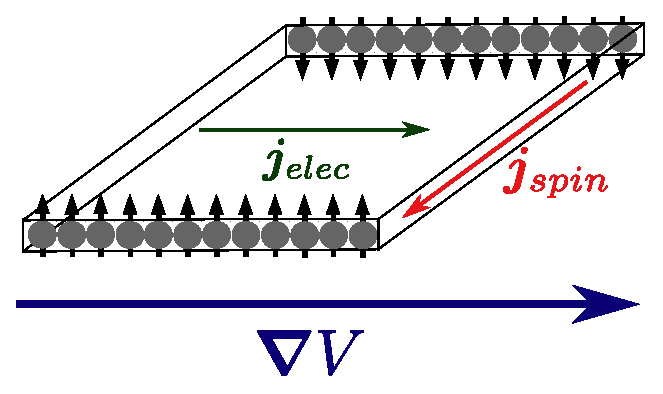
\includegraphics[width=0.5\linewidth]{./Illustrations/SHE_electrons.eps}
			\caption{Illustration de l'effet Hall de spin dans un échantillon 2D métallique soumis à un gradient de potentiel électrique.}
			\label{fig:spin-Hall-effect}
		\end{minipage}
	\end{figure}
	
	Nous considérons un échantillon bidimensionnel d'un semi-conducteur soumis à une différence de potentiel électrique $\vec{\nabla} V$. L'hamiltonien d'un électrons dans ce système est alors donné par l'expression :
	\begin{equation*}
		\label{exp_hamiltonien_SHE}
		H = \frac{\vec{p}^{\, 2}}{2m_e} + q_e V(\vec{r}) + \mathcal{A}_{SO} \, (\vec{p} \wedge \! \vec{\nabla} V) \cdot \vec{S}
	\end{equation*}
	où nous avons introduit le coefficient de couplage spin-orbite $ \mathcal{A}_{SO} $ qui dépend du matériau considéré. {\color{gray} Ajouter des exemples de coefficients pour différents matériau}\\ %% TROUVER DES INFOS SUR LES COEF DE DIFFERENTS MATERIAUX
	
	Il est alors possible d'écrire des trajectoires semi-classique pour les électrons :
	\begin{align}
		& \frac{d\vec{r}}{dt} = \frac{\vec{p}}{m} - \mathcal{A}_{SO} \vec{S} \wedge \vec{\nabla} V \; , \label{eq_mvt_SHE_r} \\
		& \frac{d \vec{p}}{dt} = - q_e \vec{\nabla} V(\vec{r}) \; . \label{eq_mvt_SHE_p}
	\end{align}

	Dans ces équations, nous voyons apparaître un décalage transverse de la trajectoire des électrons proportionnel à la différence de potentiel électrique et dont le signe dépend de l'orientation du spin.
	
	
	\subsection{Propagation de la lumière dans un milieu inhomogène}
	Si le couplage spin-orbite a été initialement étudiés pour la matière, récemment l'étude de ces effets pour la lumière s'est développé, permettant entre autre de mieux comprendre des phénomènes tels que l'effet Imbert-Fedorov ou l'effet Magnus optique, qui apparaissent lors de la propagation de la lumière en milieu inhomogène.\\
	
	Les effets de couplage spin-orbite optique sont liés à l'aspect vectoriel de la lumière et nécessitent donc une description complète de celles-ci. 
	
	%Pour cela, nous allons introduire rapidement les équations de propagation du champ, puis introduire différentes grandeurs qui nous seront nécessaires à la description de la propagation d'un faisceau lumineux.
	
	\begin{encart}{Activité pédagogique : réflection de la lumière à une interface}
		Blabla
	\end{encart}
	
	\subsubsection{Propagation des ondes électromagnétique}
	Dans un milieu diélectrique (non magnétique), la relation de propagation du champ électrique est donnée, dans l'espace de pulsations, par l'équation de Helmholtz vectorielle :
	\begin{equation*}
		\label{eq_Helmholtz_vect}
		- \varDelta \vec{E}(\vec{r}, \omega) + \vec{\nabla}(\vec{\nabla}\cdot \vec{E}(\vec{r}, \omega)) = \epsilon(\vec{r}) \frac{\omega^2}{c^2} \vec{E}(\vec{r}, \omega)
	\end{equation*}
	où nous avons introduit la permittivité relative du milieu $ \epsilon(\vec{r}) $. Dans la suite, nous supposerons nos ondes monochromatique et omettrons ainsi le $\omega$ dans nos expressions.\\
	
	Dans de nombreuses situations en optique, il est habituel de considérer $ \vec{\nabla} \cdot \vec{E} \sim 0 $, ce qui permet de se placer dans une approximation scalaire de la lumière. Or comme cela a déjà été évoqué, nous avons besoin ici de considérer l'aspect vectoriel de la lumière, nous devrons donc partir de l'équation complète. Cependant avant cela, il reste intéressant de discuter du cas d'une propagation paraxiale. En effet, nous nous placerons ici à la limite de validité de ces hypothèses. L'approximation paraxiale permet de décrire la propagation d'un faisceau lumineux proche de l'axe optique (considéré dans toute la suite selon z) pour des milieux où la permittivité peut s'écrire sous la forme :
	\begin{equation*}
		\epsilon(\vec{r}) \simeq \epsilon(x,y) = \bar{\epsilon} + \delta \epsilon(x,y) \; .
	\end{equation*}

	\begin{figure}[h]
		\centering
		\begin{minipage}[c]{0.85\linewidth}
			\centering
			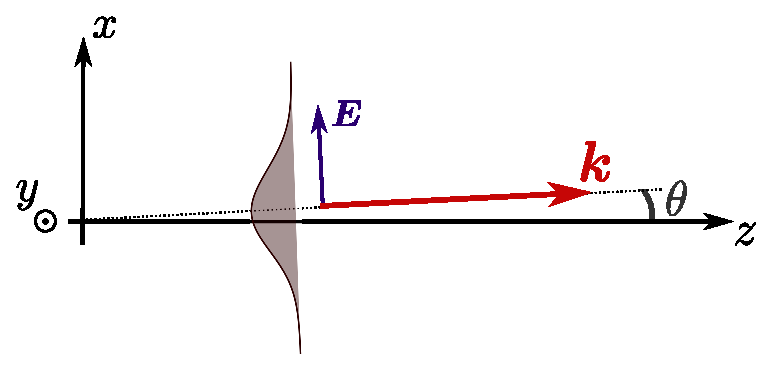
\includegraphics[width=0.65\linewidth]{./Illustrations/schema_paraxial}
			\caption{Dans l'approximation paraxiale, nous étudions des faisceaux suffisamment collimatés, dont la direction de propagation $ \vec{k} $ est faiblement inclinée par rapport à un axe optique $ z $ ($ \theta \ll 1 $) et dont la variation de l'enveloppe est suffisamment molle.}
			\label{fig:schema_paraxial}
		\end{minipage}
	\end{figure}
	
	Le champ est alors mis sous la forme :
	\begin{equation*}
		\vec{E}(\vec{r}_\perp , z) = \vec{\mathcal{E}}(\vec{r}_\perp, z) e^{i k z}
	\end{equation*}
	où nous avons introduit le vecteur position transverse $ \vec{r}_\perp = (x,y) $ et le nombre d'onde moyen $ k = \sqrt{\bar{\epsilon}} \omega / c  $. Nous supposons ici que le champ est dans le plan transverse et négligeons ainsi l'évolution de la composante longitudinale.\\
	
	L'approximation est valide pour dans l'hypothèse d'une enveloppe lentement variable, ce qui revient à considérer :
	\begin{equation*}
		\lambda \left| \frac{\vec{\nabla}\epsilon(x,y)}{\bar{\epsilon}} \right| \ll 1 \; .
	\end{equation*}
	Ces hypothèses amènent à une description scalaire de la lumière, cependant en considérant les premières corrections à l'approximation paraxiale, il est possible de décrire des effets vectoriels de la lumière.
	
	
	\subsubsection{Trajectoire du faisceau lumineux}
	\`A l'aide des équations de propagation, nous pouvons décrire l'évolution du champ électromagnétique, mais afin de caractériser la propagation d'un faisceau lumineux, nous allons introduire d'autres grandeurs qui permettent de définir une trajectoire pour la lumière. Une première quantité pertinente à considérer est le vecteur de Poynting moyen qui caractérise le transport d'énergie de l'onde électromagnétique. Son expression est donnée par
	\begin{equation*}
		\langle \vec{\Pi} \rangle (\vec{r}) = \frac{1}{2 \mu_0} \vec{E}(\vec{r}) \wedge \vec{B}^*(\vec{r}) \; .
	\end{equation*}
	Ce vecteur indique alors la direction de propagation du faisceau lumineux et permet de définir une impulsion locale :
	\begin{equation*}
		\vec{p}(\vec{r}) = \epsilon_0 \mu_0 \langle \vec{\Pi} \rangle (\vec{r}) \; .
	\end{equation*}

	La trajectoire du faisceau est définie par la position son centroïde. Si nous nous plaçons dans l'approximation paraxiale introduite précédemment, cette trajectoire est donnée par :
	\begin{equation*}
		\vec{R}(z) = \frac{ \int \! dx dy \; \vec{r} \, \langle \Pi_z \rangle (\vec{r})}{\int \! dx dy \; \langle \Pi_z \rangle (\vec{r}) } \; .
	\end{equation*}

	\begin{encart}{Activité pédagogique : étude documentaire d'un mirage}
		Blabla
	\end{encart}
	
	
	\subsubsection{Moment cinétique de la lumière}
	Afin de décrire des effets de couplage spin-orbite de la lumière, nous devons évidemment à présent introduire le moment cinétique d'un faisceau lumineux. Pour cela, nous reprenons la définition du moment cinétique classique pour écrire le moment cinétique local :
	\begin{equation*}
		\vec{j}(\vec{r}) = \vec{r} \wedge \vec{p}(\vec{r}) \; .
	\end{equation*}
	
	Le moment cinétique total d'un faisceau lumineux dans l'approximation paraxiale est alors donné par :
	\begin{equation*}
		\vec{J} (z) = \int \! dx dy \; \vec{j}(\vec{r}) = \frac{\epsilon_0}{2 i \omega} \int \! dx dy \; E_i^* (\vec{r} \wedge \vec{\nabla} ) E_i + \frac{\epsilon_0}{2 i \omega} \int \! dx dy \; \vec{E}^* \! \wedge \vec{E} \; .
	\end{equation*}
	Nous voyons ainsi deux contributions au moment cinétique totale.\\
	
	\begin{figure}[h]
		\centering
		\begin{minipage}[c]{0.85\linewidth}
			\centering
			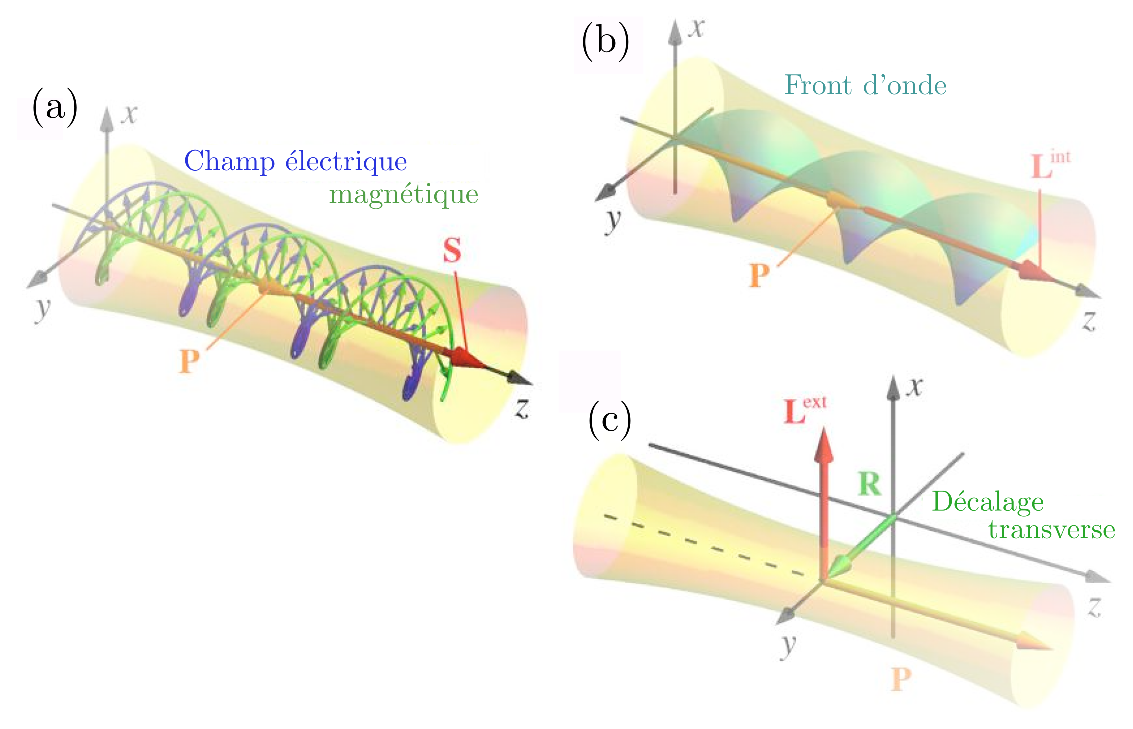
\includegraphics[width=0.9\linewidth]{./Illustrations/moments_angulaires}
			\caption{Illustrations tirées de l'article de Bliokh, Rodriguez-Fortuño, Nori et Zayats illustrant les différents moments cinétiques de la lumière : (a) le spin du faisceau lumineux, lié à la rotation des champs électrique et magnétique ; (b) le moment cinétique orbital intrinsèque, lié à une variation de la phase du champ ; (c) le moment cinétique orbital extrinsèque, lié à un déplacement du faisceau lumineux par rapport à une origine. Ici, la notation $ \vec{P} $ correspond à l'impulsion moyenne du faisceau.}
			\label{fig:moments_angulaires}
		\end{minipage}
	\end{figure}
	
	La première dépend de la variation spatiale du champ électromagnétique et donc du faisceau. On l'interprète ainsi comme un moment cinétique orbital et on le note :
	\begin{equation*}
		\vec{L}(z) = \frac{\epsilon_0}{2 i \omega} \int \! dx dy \; E_i^* (\vec{r} \wedge \vec{\nabla} ) E_i
	\end{equation*}
	Celui-ci décrit deux phénomènes différents : une déformation du front d'onde du faisceau, on parle alors de moment cinétique orbital intrinsèque, ou un déplacement de faisceau pour lequel on parle de moment cinétique orbital extrinsèque. Dans le cadre de ce dossier, c'est ce dernier qui va nous intéresser.\\
	
	Le second terme lui dépend de la valeur locale du champ électrique et plus particulièrement de la nature de sa polarisation. En effet, on voit que ce terme est non-nul si et seulement si la partie imaginaire du champ électrique est non-nulle, c'est-à-dire si l'on a une polarisation tournante. Cette contribution s'interprète alors comme un moment cinétique de spin que l'on note :
		\begin{equation*}
			\frac{\epsilon_0}{2 i \omega} \int \! dx dy \; \vec{E}^* \! \wedge \vec{E}
		\end{equation*}
	Dans le cas d'un faisceau collimaté de vecteur d'onde moyen $ \vec{K} $, ce dernier peut s'écrire sous la forme simple :
	\begin{equation*}
		\vec{S} = \frac{\epsilon_0 I}{\omega} \; \sigma \, \vec{e}_{\vec{K}}
	\end{equation*}
	où nous avons introduit l'intensité du faisceau $ I = \int dx dy |\vec{E}|^2 $, sa direction de propagation $ \vec{e}_{\vec{K}} = \vec{K} / \| \vec{K} \| $ et son hélicité $ \sigma = 2 \text{Im}(E_x^* E_y) / |\vec{E}|^2 $. Celle-ci varie entre 0 pour un polarisation rectiligne et $\pm 1 $ pour une polarisation circulaire, les valeurs intermédiaires caractérisant une polarisation elliptique.
	
	\subsubsection{Effet de couplage spin-orbite optique}
	La discussion sur des effets de couplages spin-orbite de la lumière est assez récente (début des années 2000) mais elle a permis de réinterpréter des effets décrits dès les années 70 tels que l'effet Imbert-Fedorov et l'effet Magnus optique. Ce dernier décrit une déviation transverse d'un faisceau polarisé circulairement au sein d'un milieu inhomogène et a été dérivé en prenant en compte les premières déviations à l'approximation paraxiale. La trajectoire du faisceau est alors décrite par le système  d'équation :
	\begin{align}
		& \frac{d \vec{R} }{dz} = \vec{e}_{\vec{K}} - \frac{\sigma}{K} \left[ \vec{e}_{\vec{K}} \wedge \vec{\nabla}( \ln n ) \right] \; , \label{effet_Magnus_optique2} \\
		& \frac{d \vec{K}}{dz} = \vec{\nabla} \ln n \; .
	\end{align}
	Mises sous cette forme, nous voyons bien apparaître ici l'analogie avec les équations de l'effet Hall de spin des électrons. Une différence notable avec ce dernier est cependant que le couplage spin-orbite optique apparaît spontanément dès l'existence d'une inhomogénéité dans le milieu.
	
	\begin{figure}[h]
		\centering
		\begin{minipage}[c]{0.85\linewidth}
			\centering
			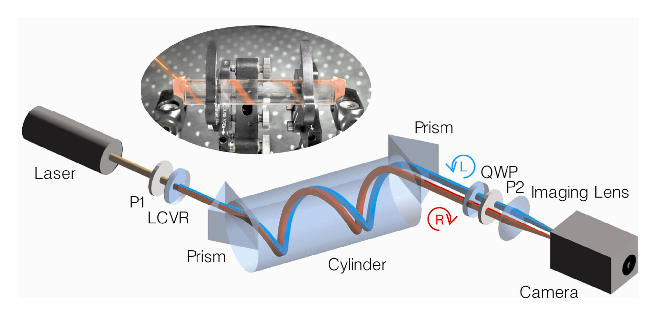
\includegraphics[width=0.9\linewidth]{./Illustrations/Bliokh_mesure_SHE-light-1.eps}
			\caption{Figures tirées de l'article de Bliokh, Niv, Kleiner et Hasman. Schéma du montage expérimental utilisé pour mesurer les décalages transverses liés à l'effet Hall de spin optique : un faisceau laser polarisé circulairement est envoyé en incidence rasante sous la surface d'un cylindre au sein duquel il suit une trajectoire hélicoïdale. La position du faisceau à la sortie est mesurée à l'aide du caméra. L'angle d'incidence du laser permet de contrôler le nombre de tours effectués par le faisceau au sein du cylindre.}
			\label{fig:mesure_SHE_light}
		\end{minipage}
	\end{figure}
	
	\subsection{Effet Hall de spin optique en désordre transverse}
	\subsubsection{Propagation dans un système désordonné}
	
	\begin{figure}[h]
		\centering
		\begin{minipage}[c]{0.85\linewidth}
			\centering
			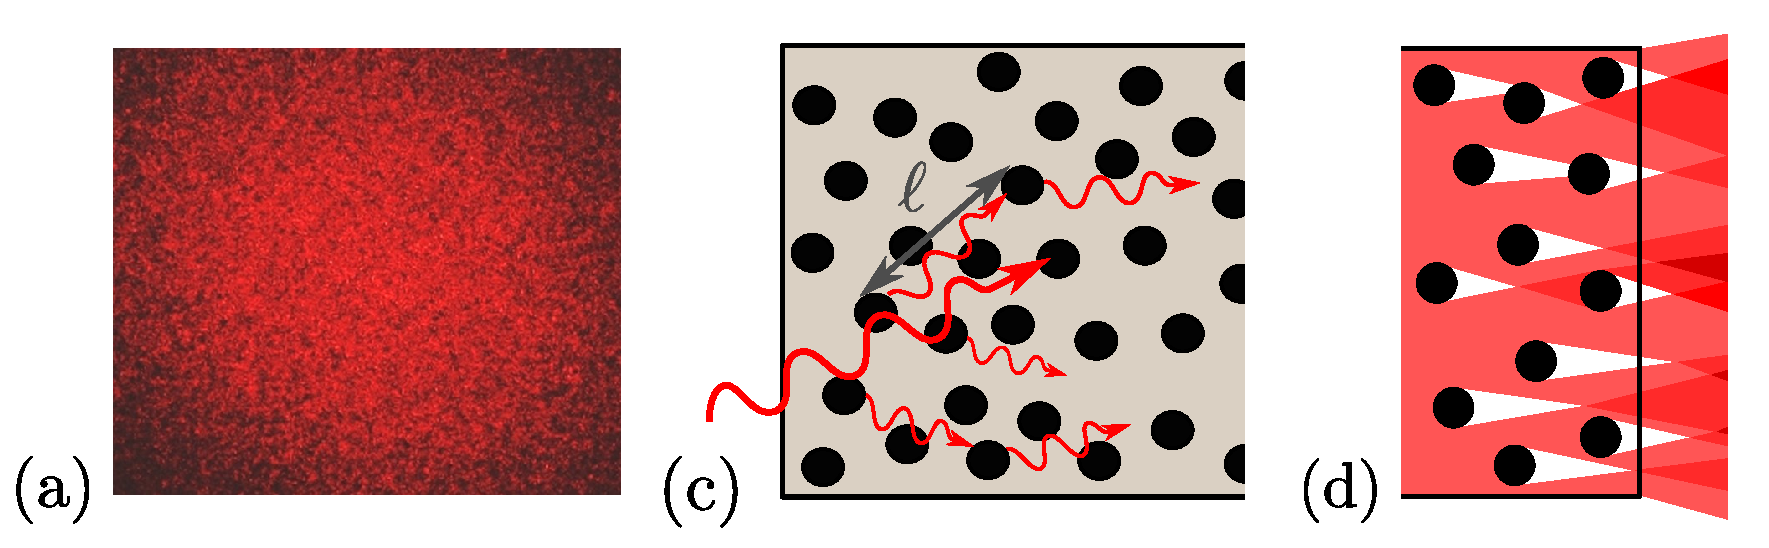
\includegraphics[width=0.85\linewidth]{./Illustrations/figure_scatt.eps} \\
			(b) \hspace{0.1cm} \includegraphics[width=0.8\linewidth]{./Illustrations/Photo_diff_desordre_3D}
			\caption{(a) Photo d'un speckle produit par un faisceau laser après propagation au travers d'un morceau de plastique rugueux. (b) Photo du phénomène de diffusion multiple dans un milieu diffusant (ici de l'eau contenant un peu de maïzena en suspension). (c) Schéma de la diffusion de la lumière se propageant à travers une distribution aléatoire de diffuseurs. (d) Schéma de la lumière diffusée à la sortie du milieu.}
			\label{fig:diffusion_desordre_3D}
		\end{minipage}
	\end{figure}

	Les milieux dits désordonnés sont des milieux très inhomogènes où l'indice optique varie de manière aléatoire. Cela va correspondre par exemple à des poudres, du verre dépoli ou des solutions contenant des particules en suspensions. Lorsqu'un faisceau lumineux se propage dans de tels milieux, nous pouvons observer différents phénomènes illustrés sur la figure \ref{fig:diffusion_desordre_3D}. Si l'on observe le comportement de la lumière au sein du milieu (comme montré sur la figure \ref{fig:diffusion_desordre_3D}(b) ), nous pouvons tout d'abord décrire deux  composantes différentes :
	\begin{itemize}
		\item le faisceau balistique qui décrit la trajectoire que l'on attendrait en absence de désordre. Son intensité décroit de manière exponentielle lors de la propagation dans le milieu.
		\item le halo diffusif qui lui apparaît autour du faisceau balistique au cours de la propagation.
	\end{itemize}
	Ces comportements sont dus à la diffusion de la lumière de la lumière sur les petits obstacles qui sont à l'origine de l'inhomogénéité du milieu. La longueur caractéristique de la diffusion qui apparaît est alors la distance moyenne entre deux processus de diffusion appelée libre parcours moyen. Si on considère une lumière cohérente, les composantes du halo diffusif se propageant dans différentes directions vont interférer, on voit alors apparaître un profil d'intensité désordonné appelée \textit{speckle}, avec des tâches lumineuses entourées de zones plus sombres comme présenté sur la figure \ref{fig:diffusion_desordre_3D}(a).
	
	
	Afin de pouvoir décrire analytiquement ce problème, nous nous basons sur une approche statistique à l'aide du formalisme du tenseur de Green. Nous considérons l'équation d'Helmholtz vectorielle que nous écrivons sous la forme :
	\begin{equation*}
		\Delta \vec{E}(\vec{r}) - \vec{\nabla}(\vec{\nabla} \cdot \vec{E}(\vec{r})) - V(\vec{r}) \vec{E}(\vec{r}) = - k^2 \vec{E}
	\end{equation*}
	où nous avons introduit $ k^2 = \bar{\epsilon} \; \omega^2 / c^2 $ qui représente le nombre d'onde moyen dans le milieu, et $ V(\vec{r}) = - k^2 \delta \epsilon(\vec{r}) / \bar{\epsilon} $ qui peut être vu comme un potentiel désordonné effectif dans lequel la lumière évolue.\\
	
	Les calculs du tenseur de Green permet alors d'étudier la propagation du champ électrique moyenné sur les réalisations du désordre. Ce champ moyen décrit alors le faisceau balistique.
	
	
	\subsubsection{Cas du désordre transverse}
	
	Lors de ma thèse, j'ai étudié les effets de couplage spin-orbite de la lumière dans les milieux désordonnés. Il s'agit à notre connaissance des premières investigations à ce sujet. Ces effets apparaissent uniquement dans des milieux où il existe une certaine anisotropie, nous avons donc considéré un désordre dit transverse. C'est-à-dire un milieu où la permittivité est homogène selon l'axe $ z $ mais varie aléatoirement dans le plan $ (x,y) $, comme représenté sur la figure \ref{fig:systeme_desordre_transverse}. Nous allons y décrire la propagation d'un faisceau gaussien collimaté arrivant avec un léger angle dans le plan $ (x,z) $ et dont la polarisation initiale est décrite par le vecteur $ \vec{\varepsilon} $ (réel pour une polarisation rectiligne et complexe pour une polarisation elliptique). Nous nous plaçons proche de l'approximation paraxiale, cependant, à l'aide du formalisme du tenseur de Green, nous pouvons étudier les premières corrections liées à l'aspect vectoriel.
	
	\begin{figure}[h]
		\centering
		\begin{minipage}[c]{0.85\linewidth}
			\centering
			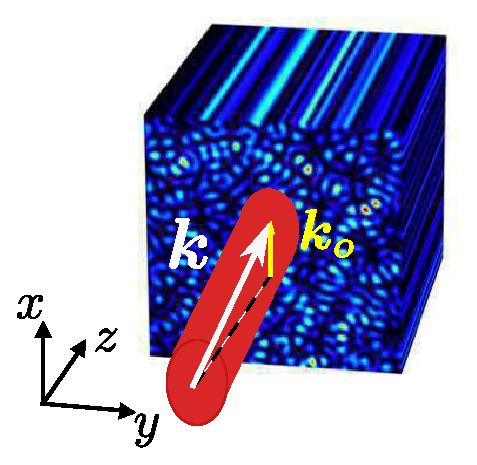
\includegraphics[width=0.35\linewidth]{./Illustrations/2+1disorder.eps}
			\caption{Illustration d'un milieu désordonné dans le plan transverse $ (x,y) $ et homogène selon l'axe optique $ z $, sur lequel est envoyé un faisceau lumineux collimaté \textit{tilté}, de vecteur d'onde transverse $ \vec{k}_0 $ selon $ \vec{e}_x $.}
			\label{fig:systeme_desordre_transverse}
		\end{minipage}
	\end{figure}
	
	Dans ce cadre, nous obtenons, pour le champ moyen, l'expression dans l'espace des impulsions :
	\begin{equation*}
		\langle \vec{E} (\vec{q}_\perp, z) \rangle = w_0\sqrt{\pi} \; e^{-\frac{w_0^2}{8} (\vec{q}_\perp - \vec{k}_0)^2 } \; e^{i k_0 x} \, e^{i k_z z} e^{- \frac{z}{z_s}} \left[ \vec{\varepsilon} - \left( 1 - e^{\frac{z}{z_{\text{\tiny SH}}}} \right) (\varepsilon_\perp \vec{e}_\perp + \varepsilon_z \vec{e}_z) \right]
	\end{equation*}
	où nous avons introduit deux longueurs caractéristiques :
	\begin{itemize}
		\item une longueur de diffusion $ z_s $ qui dépend des corrélations du désordre et de la longueur d'onde de la lumière (et qui est caractéristique de la propagation dans un milieu désordonné),
		\item une longueur caractéristique de l'effet Hall de spin $ z_\text{\tiny SH} = \frac{2k}{k_0} z_s $ .
	\end{itemize}
	
	
	\subsubsection{Trajectoire du faisceau}
	
	Ayant obtenu le champ moyen, nous pouvons obtenir la trajectoire du faisceau balistique caractérisée par la position du centroïde dans le plan $ (x,y) $ :
	\begin{equation*}
		\vec{R}_\perp (z) = \frac{\vec{k}_0}{k} z - \frac{\sigma}{k} \left[ 1 - \frac{1}{\cosh (z/z_\text{\tiny SH})} \right] \vec{e}_y \; .
	\end{equation*}
	Nous voyons ici deux termes, le premier correspond à la propagation balistique attendue sans la prise en compte des effets de couplage spin-orbite. Le terme supplémentaire décrit quant à lui un déplacement latéral (noté $ \delta R_\perp $), de l'ordre de la longueur d'onde transverse et proportionnel à l'hélicité du faisceau. On retrouve ainsi un résultat analogue à un effet Hall de spin optique.
	
	\begin{figure}[h]
		\centering
		\begin{minipage}[c]{0.85\linewidth}
			\centering
			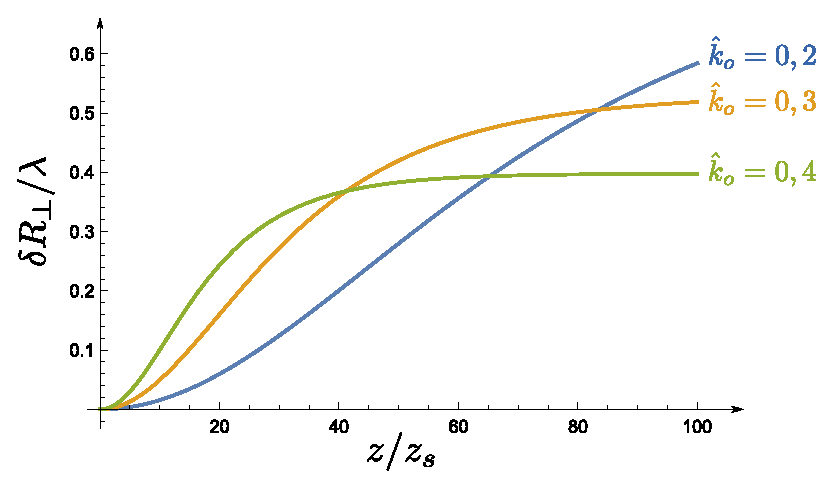
\includegraphics[width=0.8\linewidth]{./Illustrations/Plot_delta-R}
			\caption{Graphe de l'évolution du déplacement $ \delta R_\perp $ en fonction de $ z $ pour différentes valeurs de l'angle d'incidence $ k_0/k $}
			\label{fig:Plot_delta-R}
		\end{minipage}
	\end{figure}
	
	De plus, on voit apparaître un effet de saturation du décalage. Pour comprendre cela, nous nous allons nous intéresser à l'évolution du moment cinétique.
	
	
	\subsubsection{\'Evolution du moment cinétique}
	\`A nouveau, en utilisant l'expression du champ électrique moyen, nous pouvons calculer l'expression des moments cinétiques du faisceau lumineux. Le moment cinétique orbital est alors donné par :
	\begin{equation*}
		\label{exp_L(z)}
		\vec{L}(z) = \left(\vec{R}_\perp(z) + z \, \vec{e}_z \right) \wedge ( \vec{k}_0 + k_z \vec{e}_z ) 
	\end{equation*}
	où nous reconnaissons alors la forme classique bien connue $ \vec{L} = \vec{R} \wedge \vec{p} $ où $ \vec{p} = \vec{k}_0 + k_z \vec{e}_z $.\\
	
	Le spin est lui donné par l'expression :
	\begin{equation}
		\label{exp_S(z)}
		\vec{S}(z) =  \frac{ \sigma \, \frac{\vec{k}}{k} }{ \cosh \left( z/z_\text{{\tiny SH}} \right) } \; .
	\end{equation}
	
	Leur évolution est alors tracée sur le graphe présenté figure \ref{fig:conversion_moment_cinetique} pour une polarisation initiale circulaire. Nous voyons ainsi que le moment cinétique de spin diminue tandis que le moment orbital augmente (le moment cinétique total selon $ z $ reste lui constant). Cela s'explique par un transfert de moment cinétique causé par une déformation de la polarisation du faisceau au fur et à mesure de la propagation dans le milieu désordonné.
	
	\begin{figure}[h]
		\centering
		\begin{minipage}[c]{0.85\linewidth}
			\centering
			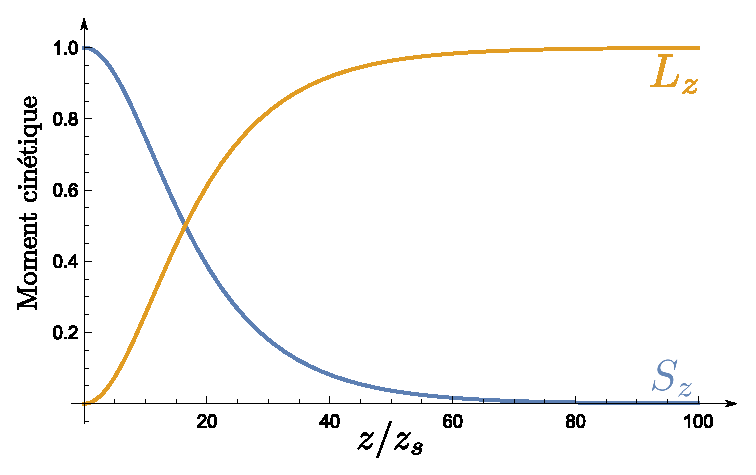
\includegraphics[width=0.7\linewidth]{./Illustrations/Plot_conversion_L-S.eps}
			\caption{Courbes des composantes $ S_z $ et $ L_z $ des moments cinétiques en fonction du temps $ z $ pour $ \sigma = + 1 $ et $ k_0 / k = 0.4 $. \`{A} l'instant initial, le système possède uniquement un moment cinétique de spin qui est converti au fur et à mesure de la propagation en moment cinétique orbital, la somme $ L_z + R_z $ restant constante.}
			\label{fig:conversion_moment_cinetique}
		\end{minipage}
	\end{figure}
	
	\section{Valorisation dans l'enseignement}
	Lors de ma thèse, j'ai pu étudier des situations très variées de propagation dans des milieux complexes, or la lumière est centrale en physique. Je pourrais ainsi exploiter les différentes connaissances que j'ai pu acquérir pour essayer de faire comprendre des éléments d'optique aux élèves.\\
	
	J'ai également eu l'occasion d'étudier des systèmes quantiques ou des analogues à des systèmes. La physique quantique prenant une place de plus en plus centrale dans notre vie et dans les programmes scolaires, ainsi que dans les médias et sur internet, où de nombreux éléments de désinformation peuvent circuler. Il est donc important, à mon avis, de pouvoir discuter de ces sujets avec les élèves en ayant des bases assez solides.
	
	
	\section{Enseignement et médiation scientifique}
	\subsection{Monitorat au sein de Sorbonne Université}
	Durant mes trois années de thèse, j'ai effectué un monitorat au sein de l'université Sorbonne Université. L'enseignement était déjà quelque chose qui me tenait à cœur avant cela, en effet, j'ai toujours considéré que la transmission des connaissances est une étape essentielle de l'apprentissage personnel. C'est pour cela qu'il était très important pour moi de pouvoir compléter mon travail de recherche au cours de ma thèse par des enseignements. Mon monitorat a confirmé ma vocation de professeure.\\ 
	
	J'ai encadré des groupes de travaux dirigés de mécanique en L2 pendant lesquels j'ai pû développer mes capacités de calculs au tableau et une approche pédagogique insistant sur l'importance pour les étudiant\pointmedian es de pouvoir poser des questions. J'y ai également appris à gérer mon planning, devant balancer la contrainte du programme (et des examens) avec un rythme permettant aux étudiant\pointmedian es de bien saisir les notions importantes et de s'approprier les outils vu en cours.\\
	
	J'ai également encadré des groupes de travaux pratiques d'optique. Ici, le format en demi-groupe et avec des binômes amenait à un encadrement plus proche et permettant de discuter plus en profondeur les notions physiques avec les étudiant\pointmedian es. Pendant ces séances, j'ai également dû gérer une évaluation continue des étudiant\pointmedian es par la correction de comptes-rendus ainsi que par la tenue d'interrogations rapides à chaque séance.\\
	
	\subsection{Participation au tournoi de physique}
	Au cours de mon cursus à Sorbonne Université j'ai pris part au \textit{French Physicists' Tournament} (qui constitue la sélection française de l'\textit{International Physicists' Tournament}). Durant celui-ci, des équipes, issues de différentes universités et écoles, se retrouvent pour \textgravedbl s'affronter\textacutedbl{} sur des problèmes de physique ludiques où elles doivent présenter et critiquer les résultats qu'elles ont obtenus durant un semestre de travail. Il s'agit d'un moment de nombreuses discussions physiques, ainsi qu'une première expérience du travail de recherche pour de nombreu\pointmedian es étudiant\pointmedian es.\\
	
	J'ai tout d'abord participé en tant que membre de l'équipe durant ma première année de master. Comme pour beaucoup, cela a été pour moi l'une des premières occasions où j'ai pu étudier en très grande autonomie un sujet de physique, mais cela a surtout été une première expérience de présentation de mes résultats personnels et du travail d'un semestre entier sur un temps de 10 minutes, pendant cette présentation il fallait ainsi être pédagogique (le jury composé de physicien\pointmedian nes ne connaissant pas spécialement les sujets) et présenter correctement sa démarche et ses résultats tout en restant très concis.\\
	
	J'ai ensuite eu l'occasion durant mon monitorat d'encadrer l'équipe de Sorbonne Université. J'ai pu y transmettre ma propre expérience du tournoi, ainsi que de discuter avec des étudiant\pointmedian es en master du travail de recherche et de la démarche scientifique. L'encadrement de tels projets est très particulier, en effet, les étudiant\pointmedian es doivent construire elleux-même leur démarche, et nous cherchions à leur donner le plus d'autonomie possible, il fallait donc accompagner les étudiant\pointmedian es et être prêt\pointmedian es à répondre à leurs questions sans essayer de les guider dans une direction particulière. Il s'agit aussi d'une expérience d'enseignement où il est nécessaire de jongler entre de nombreux domaines de la physique.\\
	
	\`A présent je participe à l'organisation de ce tournoi qui est également un grand moment de partage scientifique en tout genre. Il s'agit de réfléchir à la sélection des sujets pour le tournoi français, en équilibrant les divers domaines, mais également les types d'approches que les questions vont demander (expérience de coin de table, simulations, traitement de données, problème d'ingénierie, etc.). Il y a également de nombreuses questions de logistique à gérer.
	
	
	\subsection{Vulgarisation scientifique}
	Au cours de mon stage de M2, puis de ma thèse j'ai pu participer au stand du Laboratoire Kastler Brossel de la Fête de la Science sur le campus Pierre et Marie Curie. Au sein de celui-ci, nous présentions de nombreuses expériences autour de la lumière, allant d'une \textgravedbl simple\textacutedbl{} mesure de la vitesse de la lumière à la production d'un laser en passant par les phénomènes d'interférences, ainsi que la démonstration historique de Kastler sur l'absorption et l'émission du sodium. De plus, nous recevons des publics très variés allant de classes de primaire à des universitaires, cela m'a ainsi appris à adapter mon discours et ma pédagogie aux personnes en face de moi et en fonction de la difficulté des sujets. Nous devions également gérer des questions de temps soit dans le cas de groupes scolaires qui étaient sur un planning précis, soit car le laboratoire organisait également des visites qui partaient à intervalles réguliers du stand. Ayant participé à trois reprises à la Fête, je connaissais très bien le stand et je faisais partie de l'équipe préparation et installation.
	
	\subsection{Autres activités}
	Durant mes années d'études à Sorbonne Université, j'ai également pris une part très active dans l'association des étudiant\pointmedian es de physique CurieOsity.\\ 
	Au sein de celle-ci, j'ai pu participé à l'organisation de séances de tutorat, durant lesquelles des étudiant\pointmedian es de licences voire de master pouvaient venir librement pour demander de l'aide sur certains sujets. Cela nous forçait en tant qu'encadrant\pointmedian es à devoir comprendre efficacement et en un temps court les différents sujets pour pouvoir les expliquer clairement, en s'adaptant au niveau de l'étudiant\pointmedian e concerné\pointmedian e. Cela nous obligeait ainsi également à avoir en tête les différents programmes de l'université.\\
	Nous organisions aussi des rencontres entre chercheur\pointmedian euses et étudiant\pointmedian es sous un format un peu informel appelé les \textit{cafés-prof} pendant lesquels les professeur\pointmedian es pouvaient présenter leur domaine de recherche mais également leur parcours. Nous avons également organisé des conférences plus traditionnelles.\\
	L'association était aussi une interlocutrice privilégiée des équipes pédagogiques de l'université. Nous étions ainsi contacté pour discuter des envies et des besoins des étudiant\pointmedian es, ou pour faire le pont avec l'administration dans certaines situations. En particulier, nous avions participé à l'élaboration de la nouvelle maquette du master.\\
	
	Je me suis également investie personnellement au sein des structures l'université, tout d'abord pendant mon master au sein du conseil de l'UFR, puis en tant que représentante des doctorant\pointmedian es au conseil de l'école doctorale.
	
	
\end{document}
